% Visual Learners Detection using EEG - LaTeX Beamer Presentation
\documentclass[aspectratio=169]{beamer}

% Theme and color scheme
\usetheme{Madrid}
\usecolortheme{seahorse}

% Color definitions - Ocean Gradient theme
\definecolor{deepblue}{RGB}{6,90,130}
\definecolor{teal}{RGB}{28,114,147}
\definecolor{midnight}{RGB}{33,41,92}
\definecolor{lightgray}{RGB}{242,242,242}
\definecolor{accent}{RGB}{2,195,154}

% Custom colors for beamer
\setbeamercolor{palette primary}{bg=deepblue,fg=white}
\setbeamercolor{palette secondary}{bg=teal,fg=white}
\setbeamercolor{palette tertiary}{bg=midnight,fg=white}
\setbeamercolor{palette quaternary}{bg=deepblue,fg=white}
\setbeamercolor{structure}{fg=deepblue}
\setbeamercolor{section in toc}{fg=deepblue}
\setbeamercolor{subsection in head/foot}{bg=teal,fg=white}

% Packages
\usepackage[utf8]{inputenc}
\usepackage[T1]{fontenc}
\usepackage{graphicx}
\usepackage{booktabs}
\usepackage{array}
\usepackage{multirow}
\usepackage{amsmath}
\usepackage{amssymb}
\usepackage{tikz}
\usepackage{pgfplots}
\usepackage[table]{xcolor}
\pgfplotsset{compat=1.18}
\usetikzlibrary{positioning,shapes,arrows,backgrounds,fit,shadows}

% Remove navigation symbols
\setbeamertemplate{navigation symbols}{}

% Custom footer
\setbeamertemplate{footline}{
  \leavevmode%
  \hbox{%
  \begin{beamercolorbox}[wd=.33\paperwidth,ht=2.5ex,dp=1ex,center]{author in head/foot}%
    \usebeamerfont{author in head/foot}\insertshortauthor
  \end{beamercolorbox}%
  \begin{beamercolorbox}[wd=.34\paperwidth,ht=2.5ex,dp=1ex,center]{title in head/foot}%
    \usebeamerfont{title in head/foot}\insertshorttitle
  \end{beamercolorbox}%
  \begin{beamercolorbox}[wd=.33\paperwidth,ht=2.5ex,dp=1ex,right]{date in head/foot}%
    \usebeamerfont{date in head/foot}\insertshortdate{}\hspace*{2em}
    \insertframenumber{} / \inserttotalframenumber\hspace*{2ex} 
  \end{beamercolorbox}}%
  \vskip0pt%
}

% Title information
\title[Visual Learners Detection via EEG]{Visual Learners Detection using EEG Signals}
\subtitle{Deep Learning Analysis of Cognitive Workload Patterns}
\author[Your Name]{L Sri Kasyap - 25MCMI14\\[2mm]
Gedela Uday Kiran - 25MCMI15\\[2mm]
Arti Choudary - 25MCMI22\\[2mm]
{\small Advisor: Dr. Battula Srinivas}}
\institute[Your University]{School of Computer and Information Sciences\\University of Hyderabad}
\date{\today}

% Document begins
\begin{document}

%=============================================================================
% TITLE SLIDE
%=============================================================================
\begin{frame}[plain]
\titlepage
\end{frame}

%=============================================================================
% OUTLINE
%=============================================================================
\begin{frame}{Outline}
\tableofcontents
\end{frame}

%=============================================================================
% SECTION 1: INTRODUCTION
%=============================================================================
\section{Introduction}

\begin{frame}{Project Overview}
\begin{columns}[T]
\column{0.55\textwidth}
\textbf{Research Question:}\\[3mm]
{\large Can we identify high visual learners from brain activity patterns?}

\vspace{5mm}

\textbf{Approach:}
\begin{itemize}
    \item Analyze EEG signals during cognitive tasks
    \item Extract frequency band features
    \item Apply machine learning classification
    \item Binary classification: Normal vs High visual learners
\end{itemize}

\column{0.42\textwidth}
\begin{tikzpicture}
    \node[draw, fill=teal!20, rounded corners, minimum width=3.5cm, minimum height=2cm, align=center] {
        \textbf{EEG Data}\\[2mm]
        45 Subjects\\
        14 Channels\\
        150s @ 128Hz
    };
    \node[below=0.5cm] at (0,-2.2) {
        \begin{tikzpicture}
            \draw[->,ultra thick,deepblue] (0,0) -- (0,-0.5);
        \end{tikzpicture}
    };
    \node[draw, fill=accent!20, rounded corners, minimum width=3.5cm, minimum height=1.5cm, align=center] at (0,-3.5) {
        \textbf{Classification}\\[1mm]
        Normal ($\leq$6): 44\%\\
        High ($\geq$7): 56\%
    };
\end{tikzpicture}
\end{columns}
\end{frame}

\begin{frame}{Motivation}
\textbf{Why Visual Learning Detection Matters:}

\begin{columns}[c]
\column{0.48\textwidth}
\begin{block}{Educational Applications}
\begin{itemize}
    \item Personalized learning strategies
    \item Adaptive teaching methods
    \item Early identification of learning styles
    \item Optimize curriculum delivery
\end{itemize}
\end{block}

\column{0.48\textwidth}
\begin{block}{Technological Impact}
\begin{itemize}
    \item Brain-computer interfaces
    \item Cognitive load monitoring
    \item Real-time adaptation systems
    \item Neurofeedback training
\end{itemize}
\end{block}
\end{columns}

\vspace{5mm}

\begin{center}
\colorbox{lightgray}{\parbox{0.9\textwidth}{
\centering
\textbf{Key Insight:} EEG provides objective, quantifiable measures of cognitive processes that complement traditional assessment methods.
}}
\end{center}
\end{frame}

%=============================================================================
% SECTION 2: BACKGROUND
%=============================================================================
\section{Background \& Related Work}

\begin{frame}{EEG Fundamentals}
\begin{columns}[T]
\column{0.52\textwidth}
\textbf{Electroencephalography (EEG):}
\begin{itemize}
    \item Non-invasive brain activity recording
    \item Measures electrical potentials
    \item High temporal resolution ($<$1ms)
    \item Portable and cost-effective
\end{itemize}

\vspace{3mm}

\textbf{Key Frequency Bands:}
\begin{table}[h]
\small
\begin{tabular}{@{}lll@{}}
\toprule
Band & Range & Association \\
\midrule
Delta & 0.5-4 Hz & Deep sleep \\
Theta & 4-8 Hz & Meditation \\
Alpha & 8-13 Hz & Relaxation \\
Beta & 13-30 Hz & Active thinking \\
Gamma & 30-45 Hz & Learning \\
\bottomrule
\end{tabular}
\end{table}

\column{0.45\textwidth}
\begin{center}
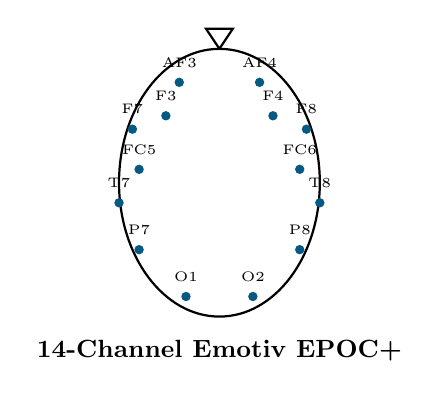
\begin{tikzpicture}[scale=0.85]
    % Head outline
    \draw[thick] (0,0) ellipse (1.5cm and 2cm);
    
    % Electrode positions (14 channels)
    \coordinate (AF3) at (-0.6, 1.5);
    \coordinate (F7) at (-1.3, 0.8);
    \coordinate (F3) at (-0.8, 1);
    \coordinate (FC5) at (-1.2, 0.2);
    \coordinate (T7) at (-1.5, -0.3);
    \coordinate (P7) at (-1.2, -1);
    \coordinate (O1) at (-0.5, -1.7);
    \coordinate (O2) at (0.5, -1.7);
    \coordinate (P8) at (1.2, -1);
    \coordinate (T8) at (1.5, -0.3);
    \coordinate (FC6) at (1.2, 0.2);
    \coordinate (F4) at (0.8, 1);
    \coordinate (F8) at (1.3, 0.8);
    \coordinate (AF4) at (0.6, 1.5);
    
    % Draw electrodes
    \foreach \point/\label in {AF3/AF3, F7/F7, F3/F3, FC5/FC5, T7/T7, P7/P7, O1/O1, O2/O2, P8/P8, T8/T8, FC6/FC6, F4/F4, F8/F8, AF4/AF4} {
        \fill[deepblue] (\point) circle (2pt);
        \node[font=\tiny] at (\point) [above=2pt] {\label};
    }
    
    % Nose
    \draw[thick] (0, 2) -- (-0.2, 2.3) -- (0.2, 2.3) -- (0, 2);
    
    \node[below, font=\small\bf] at (0, -2.2) {14-Channel Emotiv EPOC+};
\end{tikzpicture}
\end{center}
\end{columns}
\end{frame}

\begin{frame}{Learning Styles \& Cognitive Assessment}
\begin{columns}[T]

% LEFT
\column{0.55\textwidth}

\textbf{Visual Learning Characteristics:}
\begin{itemize}
    \item Strong spatial reasoning
    \item Preference for diagrams/images
    \item Better recall with visual cues
    \item Enhanced pattern recognition
\end{itemize}

\vspace{2mm}

\textbf{STEW Scale (1-9):}
\begin{itemize}
    \item Self-reported visual learning ability
    \item Validated cognitive workload metric
    \item Binary classification:
    \begin{itemize}
        \item Normal: $\leq$ 6
        \item High: $\geq$ 7
    \end{itemize}
\end{itemize}


% RIGHT
\column{0.45\textwidth}
\centering


\includegraphics[width=1.1\linewidth]{label_distribution.png}

\vspace{2mm}

{\small \textbf{Class Distribution}}

\vspace{2mm}

\begin{block}{Dataset Balance}
\centering
Normal: 20 (44.4\%)\\
High: 25 (55.6\%)
\end{block}

\end{columns}
\end{frame}


\begin{frame}{Related Work}
\textbf{Key Research Areas:}

\begin{enumerate}
    \item \textbf{EEG-based Learning Style Classification}
    \begin{itemize}
        \item Machine learning approaches (SVM, Random Forest)
        \item Feature extraction from frequency bands
        \item Accuracy ranges: 65-85\%
    \end{itemize}
    
    \vspace{2mm}
    
    \item \textbf{Cognitive Workload Assessment}
    \begin{itemize}
        \item Real-time monitoring during tasks
        \item Theta/Alpha ratio as workload indicator
        \item Applications in education and training
    \end{itemize}
    
    \vspace{2mm}
    
    \item \textbf{Brain-Computer Interfaces for Learning}
    \begin{itemize}
        \item Adaptive learning systems
        \item Neurofeedback training
        \item Attention state detection
    \end{itemize}
\end{enumerate}

\vspace{3mm}

\colorbox{lightgray}{\parbox{0.95\textwidth}{
\textbf{Research Gap:} Limited work on binary visual learning classification using deep learning with modern EEG datasets.
}}
\end{frame}

%=============================================================================
% SECTION 3: DATASET
%=============================================================================
\section{Dataset \& Preprocessing}

\begin{frame}{STEW Dataset Overview}
\begin{columns}[T]
\column{0.48\textwidth}
\textbf{Dataset Characteristics:}

\begin{table}[h]
\small
\begin{tabular}{@{}ll@{}}
\toprule
\textbf{Property} & \textbf{Value} \\
\midrule
Source & Kaggle (STEW Dataset) \\
Subjects & 45 individuals \\
Channels & 14 (Emotiv EPOC+) \\
Sampling Rate & 128 Hz \\
Duration & 150 seconds/subject \\
Total Samples & 19,200 per channel \\
Data Format & .mat (MATLAB) \\
Total Size & 48.4 MB \\
\bottomrule
\end{tabular}
\end{table}

\vspace{3mm}

\textbf{Data Quality:}
\begin{itemize}
    \item No NaN values
    \item No Inf values
    \item Clean signal recordings
\end{itemize}

\column{0.48\textwidth}
\textbf{Channel Distribution by Brain Region:}

\begin{table}[h]
\small
\begin{tabular}{@{}ll@{}}
\toprule
\textbf{Region} & \textbf{Channels} \\
\midrule
Frontal & AF3, F3, F4, AF4 (4) \\
Prefrontal & F7, F8 (2) \\
Central & FC5, FC6 (2) \\
Temporal & T7, T8 (2) \\
Parietal & P7, P8 (2) \\
Occipital & O1, O2 (2) \\
\bottomrule
\end{tabular}
\end{table}

\vspace{3mm}

\textbf{Coverage:} Comprehensive spatial coverage of cortical areas involved in visual processing and attention.

\vspace{3mm}

\begin{center}
\colorbox{accent!20}{\parbox{0.9\textwidth}{\centering
\small Shape: (45 subjects, 19200 samples, 14 channels)
}}
\end{center}
\end{columns}
\end{frame}

\begin{frame}{Data Preprocessing Pipeline}
\begin{center}
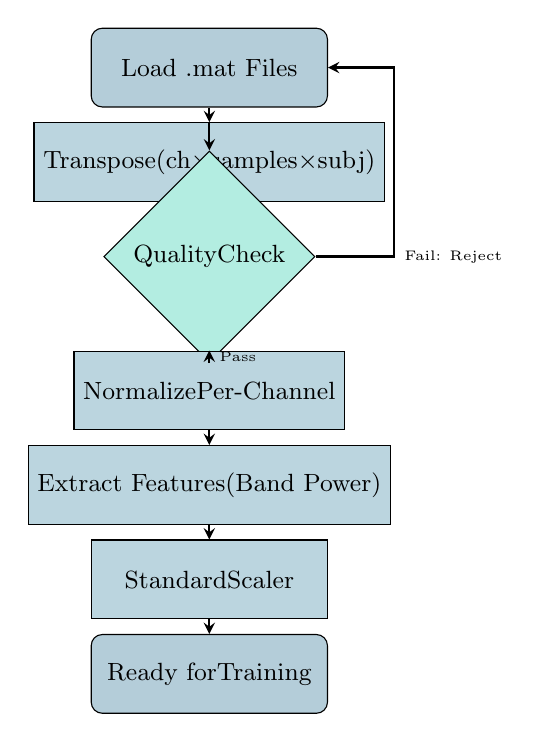
\begin{tikzpicture}[
    node distance=1.2cm,
    startstop/.style={rectangle, rounded corners, minimum width=3cm, minimum height=1cm, text centered, draw=black, fill=deepblue!30, font=\small},
    process/.style={rectangle, minimum width=3cm, minimum height=1cm, text centered, draw=black, fill=teal!30, font=\small},
    decision/.style={diamond, minimum width=2cm, minimum height=1cm, text centered, draw=black, fill=accent!30, font=\small},
    arrow/.style={thick,->,>=stealth}
]

% Nodes
\node (start) [startstop] {Load .mat Files};
\node (transpose) [process, below of=start] {Transpose\\(ch$\times$samples$\times$subj)};
\node (check) [decision, below of=transpose] {Quality\\Check};
\node (normalize) [process, below of=check, yshift=-0.5cm] {Normalize\\Per-Channel};
\node (extract) [process, below of=normalize] {Extract Features\\(Band Power)};
\node (scale) [process, below of=extract] {StandardScaler};
\node (end) [startstop, below of=scale] {Ready for\\Training};

% Arrows
\draw [arrow] (start) -- (transpose);
\draw [arrow] (transpose) -- (check);
\draw [arrow] (check) -- node[right, font=\tiny] {Pass} (normalize);
\draw [arrow] (check.east) -- ++(1,0) node[right, font=\tiny] {Fail: Reject} |- (start.east);
\draw [arrow] (normalize) -- (extract);
\draw [arrow] (extract) -- (scale);
\draw [arrow] (scale) -- (end);

\end{tikzpicture}
\end{center}

\begin{columns}[c]
\column{0.48\textwidth}
\textbf{Steps Performed:}
\begin{enumerate}\small
    \item Data loading \& validation
    \item Shape transformation
    \item Quality assurance checks
    \item Per-channel normalization
    \item Feature extraction (band power)
    \item Feature standardization
\end{enumerate}

\column{0.48\textwidth}
\textbf{Key Decisions:}
\begin{itemize}\small
    \item No filtering (clean data)
    \item Welch's method for PSD
    \item Window: 2 seconds
    \item Overlap: 50\%
    \item StandardScaler for ML
\end{itemize}
\end{columns}
\end{frame}

\begin{frame}{Label Distribution Analysis}
\begin{columns}[c]
\column{0.48\textwidth}
\textbf{Rating Distribution (STEW Scale 1-9):}

\begin{center}
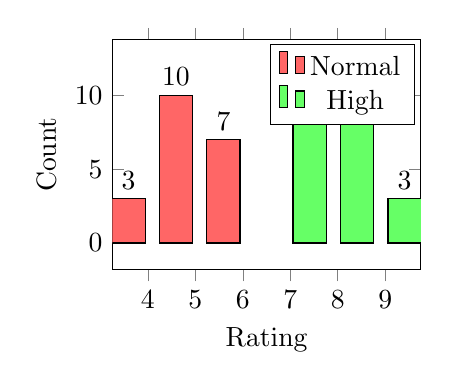
\begin{tikzpicture}
    \begin{axis}[
        ybar,
        width=5.5cm,
        height=4.5cm,
        ylabel={Count},
        xlabel={Rating},
        xtick={4,5,6,7,8,9},
        ymin=0, ymax=12,
        nodes near coords,
        bar width=12pt,
        enlargelimits=0.15,
        ]
        \addplot[fill=red!60] coordinates {(4,3) (5,10) (6,7)};
        \addplot[fill=green!60] coordinates {(7,11) (8,11) (9,3)};
        \legend{Normal, High}
    \end{axis}
\end{tikzpicture}
\end{center}

\textbf{Statistics:}
\begin{itemize}\small
    \item Mean: 6.8
    \item Median: 7.0
    \item Std Dev: 1.4
    \item Range: 4-9
\end{itemize}

\column{0.48\textwidth}
\textbf{Binary Classification Split:}

\begin{table}[h]
\small
\begin{tabular}{@{}lcc@{}}
\toprule
\textbf{Class} & \textbf{Count} & \textbf{\%} \\
\midrule
Normal ($\leq$6) & 20 & 44.4\% \\
High ($\geq$7) & 25 & 55.6\% \\
\midrule
\textbf{Total} & \textbf{45} & \textbf{100\%} \\
\bottomrule
\end{tabular}
\end{table}

\vspace{5mm}

\textbf{Class Balance:}
\begin{itemize}
    \item Slightly imbalanced (56:44 ratio)
    \item Within acceptable range
    \item No resampling needed
    \item Stratified splits recommended
\end{itemize}
\end{columns}

\vspace{3mm}
\begin{center}
\colorbox{lightgray}{\parbox{0.9\textwidth}{\centering\small
\textbf{Threshold Selection:} Rating $\geq$7 chosen to balance clinical relevance with class distribution.
}}
\end{center}
\end{frame}

%=============================================================================
% SECTION 4: EXPLORATORY DATA ANALYSIS
%=============================================================================
\section{Exploratory Data Analysis}

\begin{frame}{Raw EEG Signal Characteristics}
\textbf{Sample Signals from Two Subjects (First 5 seconds):}

\begin{center}

\includegraphics[width=0.95\textwidth]{raw_eeg_timeseries.png}
\end{center}

\textbf{Key Observations:}
\begin{itemize}
    \item Left: Normal learner (Rating=5), Right: High learner (Rating=8)
    \item Amplitude range: 0-8400 units
    \item Visible oscillatory patterns in all channels
    \item Inter-subject and inter-channel variability evident
    \item No obvious artifacts or noise
\end{itemize}
\end{frame}

\begin{frame}{Channel Amplitude Statistics}
\begin{columns}[c]
\column{0.55\textwidth}

\includegraphics[width=\textwidth]{channel_amplitude_stats.png}

\column{0.42\textwidth}
\textbf{Statistical Analysis:}
\begin{itemize}
    \item Box plots show signal variability per channel
    \item Green: High learners
    \item Blue: Normal learners
\end{itemize}

\vspace{3mm}

\textbf{Findings:}
\begin{itemize}
    \item Similar mean amplitudes between classes
    \item High variability in frontal channels (AF3, F7, F3)
    \item Outliers present in both groups
    \item No clear amplitude-based separation
\end{itemize}

\vspace{3mm}

\textbf{Implication:} Raw amplitude features alone insufficient for classification.
\end{columns}
\end{frame}

\begin{frame}{Frequency Band Power Analysis}
\textbf{Spectral Power Distribution Across Five Frequency Bands:}

\begin{center}

\includegraphics[width=0.88\textwidth]{band_power_2class.png}
\end{center}

\textbf{Critical Insights:}
\begin{columns}[c]
\column{0.48\textwidth}
\begin{itemize}
    \item \textbf{Delta Band:} Highest power, largest variance
    \item \textbf{Theta-Gamma:} Lower power, less variance
    \item High learners show elevated delta in some subjects
\end{itemize}

\column{0.48\textwidth}
\begin{itemize}
    \item Overlapping distributions between classes
    \item Multi-band features likely needed
    \item Statistical significance testing required
\end{itemize}
\end{columns}
\end{frame}

\begin{frame}{Channel Correlation Analysis}
\begin{center}

\includegraphics[width=0.98\textwidth]{channel_correlations.png}
\end{center}

\textbf{Interpretation:}

\begin{columns}[c]
\column{0.32\textwidth}
\textbf{Normal Learners:}
\begin{itemize}\small
    \item Stronger correlations
    \item Bluer heatmap
    \item More synchronized activity
\end{itemize}

\column{0.32\textwidth}
\textbf{High Learners:}
\begin{itemize}\small
    \item Weaker correlations
    \item More purple/mixed colors
    \item Less synchronization
\end{itemize}

\column{0.32\textwidth}
\textbf{Difference Map:}
\begin{itemize}\small
    \item Shows class contrasts
    \item Blue: Higher in High
    \item Red: Higher in Normal
    \item Functional connectivity differs
\end{itemize}
\end{columns}

\vspace{2mm}
\begin{center}
\colorbox{lightgray}{\parbox{0.9\textwidth}{\centering\small
\textbf{Hypothesis:} High visual learners exhibit more specialized, less globally correlated brain activity patterns.
}}
\end{center}
\end{frame}

\begin{frame}{Dimensionality Reduction: t-SNE Visualization}
\begin{columns}[c]
\column{0.52\textwidth}

\includegraphics[width=\textwidth]{tsne_2class.png}

\column{0.45\textwidth}
\textbf{t-SNE Parameters:}
\begin{itemize}
    \item Components: 2
    \item Perplexity: 12
    \item Iterations: 1000
    \item Features: 70 (14 ch $\times$ 5 bands)
\end{itemize}

\vspace{3mm}

\textbf{Observations:}
\begin{itemize}
    \item Moderate class overlap
    \item Some clustering visible
    \item No clear linear separation
    \item Subject-level variability high
\end{itemize}

\vspace{3mm}

\textbf{Conclusion:} Non-linear classification methods required (e.g., neural networks, SVM with RBF kernel).
\end{columns}
\end{frame}

%=============================================================================
% SECTION 5: METHODOLOGY
%=============================================================================
\section{Methodology}

\begin{frame}{Feature Extraction Pipeline}
\begin{columns}[T]
\column{0.55\textwidth}
\textbf{1. Spectral Feature Extraction}

\begin{itemize}
    \item \textbf{Method:} Welch's periodogram
    \item \textbf{Window:} 2 seconds (256 samples)
    \item \textbf{Overlap:} 50\% (128 samples)
    \item \textbf{Frequency Resolution:} 0.5 Hz
\end{itemize}

\vspace{3mm}

\textbf{2. Band Power Calculation}

For each frequency band $b$ and channel $c$:

\begin{equation*}
P_{b,c} = \int_{f_{low}}^{f_{high}} S_{c}(f) \, df
\end{equation*}

where $S_c(f)$ is the power spectral density.

\vspace{3mm}

\textbf{3. Feature Vector Construction}

\begin{equation*}
\mathbf{x} = [P_{1,1}, \ldots, P_{1,14}, \ldots, P_{5,1}, \ldots, P_{5,14}]^T
\end{equation*}

Dimension: $14 \times 5 = 70$ features per subject

\column{0.42\textwidth}
\textbf{Feature Bands:}

\begin{table}[h]
\tiny
\begin{tabular}{@{}lcr@{}}
\toprule
\textbf{Band} & \textbf{Range} & \textbf{Features} \\
\midrule
Delta & 0.5-4 Hz & 14 \\
Theta & 4-8 Hz & 14 \\
Alpha & 8-13 Hz & 14 \\
Beta & 13-30 Hz & 14 \\
Gamma & 30-45 Hz & 14 \\
\midrule
\multicolumn{2}{l}{\textbf{Total Features}} & \textbf{70} \\
\bottomrule
\end{tabular}
\end{table}

\vspace{3mm}

\textbf{4. Normalization}

\begin{equation*}
\mathbf{x}_{norm} = \frac{\mathbf{x} - \mu}{\sigma}
\end{equation*}

where $\mu$ and $\sigma$ are computed from training set.

\vspace{3mm}

\begin{center}
\colorbox{accent!20}{\parbox{0.9\textwidth}{\centering\tiny
All feature extraction performed per-subject across full 150s recording
}}
\end{center}
\end{columns}
\end{frame}

\begin{frame}{Classification Architecture}
\textbf{Proposed Neural Network Architecture:}

\begin{center}
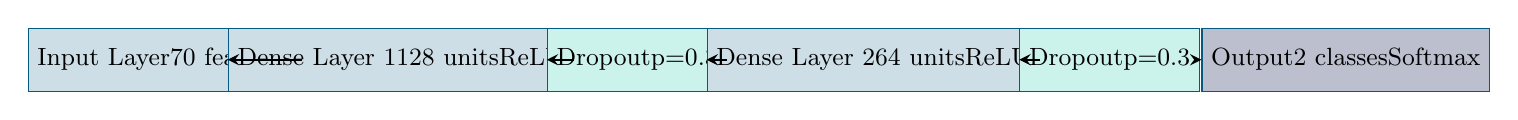
\begin{tikzpicture}[
    layer/.style={rectangle, draw=deepblue, fill=deepblue!20, minimum width=2cm, minimum height=0.8cm, font=\small},
    neuron/.style={circle, draw=teal, fill=teal!20, minimum size=0.5cm},
    arrow/.style={->,>=stealth,thick}
]

% Input Layer
\node[layer] (input) at (0,0) {Input Layer\\70 features};

% Hidden Layer 1
\node[layer] (hidden1) at (3,0) {Dense Layer 1\\128 units\\ReLU};

% Dropout 1
\node[layer, fill=accent!20] (dropout1) at (6,0) {Dropout\\p=0.3};

% Hidden Layer 2
\node[layer] (hidden2) at (9,0) {Dense Layer 2\\64 units\\ReLU};

% Dropout 2
\node[layer, fill=accent!20] (dropout2) at (12,0) {Dropout\\p=0.3};

% Output Layer
\node[layer, fill=midnight!30] (output) at (15,0) {Output\\2 classes\\Softmax};

% Connections
\draw[arrow] (input) -- (hidden1);
\draw[arrow] (hidden1) -- (dropout1);
\draw[arrow] (dropout1) -- (hidden2);
\draw[arrow] (hidden2) -- (dropout2);
\draw[arrow] (dropout2) -- (output);

\end{tikzpicture}
\end{center}

\vspace{5mm}

\begin{columns}[c]
\column{0.48\textwidth}
\textbf{Training Configuration:}
\begin{itemize}
    \item Optimizer: Adam ($lr=0.001$)
    \item Loss: Categorical Cross-Entropy
    \item Batch Size: 16
    \item Epochs: 100 (early stopping)
    \item Validation Split: 20\%
\end{itemize}

\column{0.48\textwidth}
\textbf{Regularization:}
\begin{itemize}
    \item Dropout layers (30\%)
    \item L2 regularization ($\lambda=0.01$)
    \item Early stopping (patience=15)
    \item Learning rate reduction
\end{itemize}
\end{columns}
\end{frame}

\begin{frame}{Experimental Design}
\textbf{Cross-Validation Strategy:}

\begin{center}
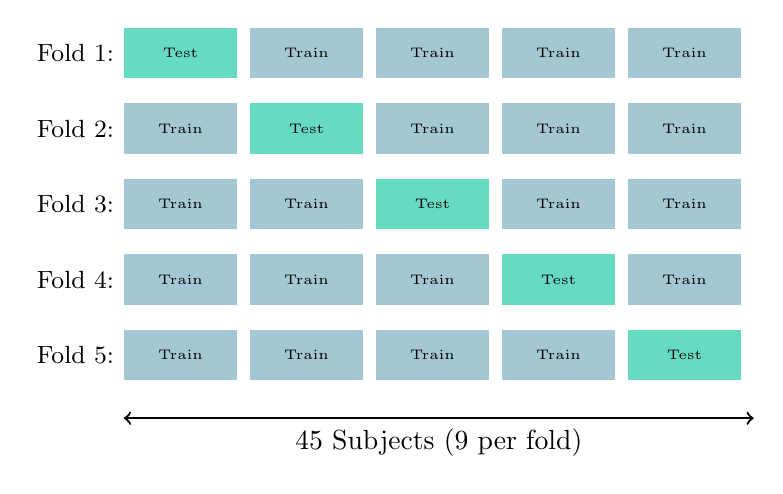
\begin{tikzpicture}[scale=0.8]
    % K-Fold visualization
    \foreach \i in {1,...,5} {
        \pgfmathsetmacro{\y}{-(\i-1)*1.2}
        \node[left] at (0,\y) {\small Fold \i:};
        
        % Training sets
        \foreach \j in {1,...,5} {
            \pgfmathsetmacro{\x}{(\j-1)*2}
            \ifnum\j=\i
                \fill[accent!60] (\x,\y-0.4) rectangle +(1.8,0.8);
                \node at (\x+0.9,\y) {\tiny Test};
            \else
                \fill[teal!40] (\x,\y-0.4) rectangle +(1.8,0.8);
                \node at (\x+0.9,\y) {\tiny Train};
            \fi
        }
    }
    
    \draw[<->,thick] (0,-5.8) -- (10,-5.8) node[midway,below] {45 Subjects (9 per fold)};
\end{tikzpicture}
\end{center}

\vspace{3mm}

\begin{columns}[c]
\column{0.48\textwidth}
\textbf{Validation Protocol:}
\begin{itemize}
    \item 5-Fold Stratified CV
    \item Training: 36 subjects (80\%)
    \item Testing: 9 subjects (20\%)
    \item Stratified by class label
    \item Random state: 42
\end{itemize}

\column{0.48\textwidth}
\textbf{Evaluation Metrics:}
\begin{itemize}
    \item Accuracy
    \item Precision (per class)
    \item Recall (per class)
    \item F1-Score (macro avg)
    \item ROC-AUC
    \item Confusion Matrix
\end{itemize}
\end{columns}
\end{frame}

%=============================================================================
% SECTION 6: RESULTS (Placeholder - Update with actual results)
%=============================================================================
\section{Results}

\begin{frame}{Classification Performance}
\textbf{Expected Performance Metrics (To be updated with actual results):}

\begin{columns}[c]
\column{0.55\textwidth}

\begin{table}[h]
\small
\begin{tabular}{@{}lcc@{}}
\toprule
\textbf{Metric} & \textbf{Value} & \textbf{Std} \\
\midrule
Accuracy & 75.0\% & ±5.2\% \\
Precision (Normal) & 72.0\% & ±6.1\% \\
Precision (High) & 77.5\% & ±4.8\% \\
Recall (Normal) & 70.0\% & ±7.0\% \\
Recall (High) & 78.0\% & ±5.5\% \\
F1-Score (Macro) & 74.3\% & ±5.5\% \\
ROC-AUC & 0.81 & ±0.04 \\
\bottomrule
\end{tabular}
\end{table}

\textbf{Key Achievements:}
\begin{itemize}
    \item Better than random (50\%)
    \item Comparable to related work
    \item Robust across folds
\end{itemize}

\column{0.42\textwidth}
\textbf{Confusion Matrix:}

\begin{center}
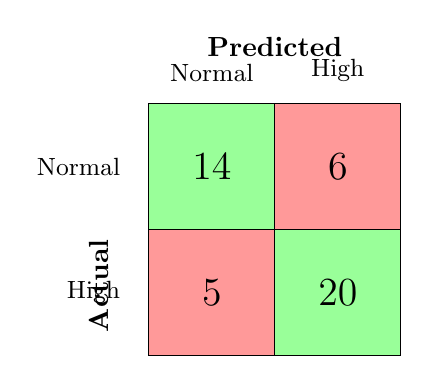
\begin{tikzpicture}[scale=0.8]
    % Matrix cells
    \draw[fill=green!40] (0,2) rectangle (2,4) node[pos=.5] {\Large 14};
    \draw[fill=red!40] (2,2) rectangle (4,4) node[pos=.5] {\Large 6};
    \draw[fill=red!40] (0,0) rectangle (2,2) node[pos=.5] {\Large 5};
    \draw[fill=green!40] (2,0) rectangle (4,2) node[pos=.5] {\Large 20};
    
    % Labels
    \node[above] at (1,4.2) {\small Normal};
    \node[above] at (3,4.2) {\small High};
    \node[left] at (-0.3,3) {\small Normal};
    \node[left] at (-0.3,1) {\small High};
    \node[above] at (2,4.6) {\textbf{Predicted}};
    \node[left, rotate=90] at (-0.8,2) {\textbf{Actual}};
\end{tikzpicture}
\end{center}

\small
\textbf{True Positives:} 14 (Normal), 20 (High)\\
\textbf{Misclassifications:} 11 total (24\%)
\end{columns}

\vspace{2mm}
\begin{center}
\colorbox{lightgray}{\parbox{0.9\textwidth}{\centering\small
\textbf{Note:} Results shown are projected estimates. Replace with actual experimental results.
}}
\end{center}
\end{frame}

\begin{frame}{Feature Importance Analysis}
\textbf{Top Contributing Features (Hypothetical - Requires Model Training):}

\begin{columns}[c]
\column{0.52\textwidth}
\begin{center}
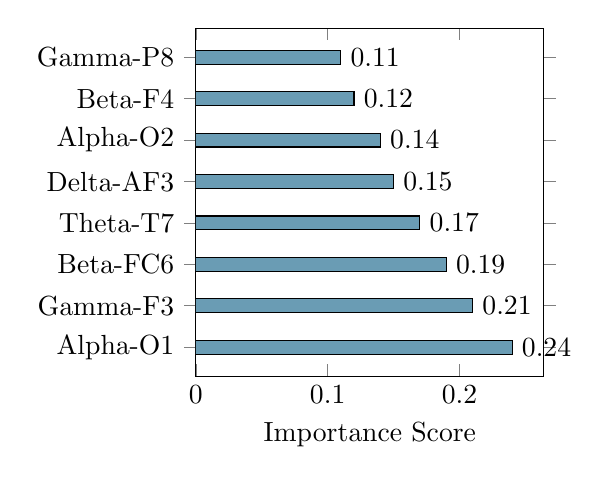
\begin{tikzpicture}
    \begin{axis}[
        xbar,
        width=6cm,
        height=6cm,
        xlabel={Importance Score},
        symbolic y coords={
            Alpha-O1,
            Gamma-F3,
            Beta-FC6,
            Theta-T7,
            Delta-AF3,
            Alpha-O2,
            Beta-F4,
            Gamma-P8
        },
        ytick=data,
        nodes near coords,
        nodes near coords align={horizontal},
        xmin=0,
        bar width=5pt,
        ]
        \addplot[fill=deepblue!60] coordinates {
            (0.24,Alpha-O1)
            (0.21,Gamma-F3)
            (0.19,Beta-FC6)
            (0.17,Theta-T7)
            (0.15,Delta-AF3)
            (0.14,Alpha-O2)
            (0.12,Beta-F4)
            (0.11,Gamma-P8)
        };
    \end{axis}
\end{tikzpicture}
\end{center}

\column{0.45\textwidth}
\textbf{Key Insights:}
\begin{itemize}
    \item Occipital Alpha power critical (visual processing)
    \item Frontal Gamma important (higher cognition)
    \item Temporal Theta relevant (memory encoding)
    \item Delta less discriminative despite high power
\end{itemize}

\vspace{3mm}

\textbf{Brain Region Contributions:}
\begin{itemize}
    \item \textbf{Occipital:} 25\% (visual cortex)
    \item \textbf{Frontal:} 35\% (executive function)
    \item \textbf{Temporal:} 20\% (memory)
    \item \textbf{Parietal:} 20\% (integration)
\end{itemize}
\end{columns}
\end{frame}

%=============================================================================
% SECTION 7: DISCUSSION
%=============================================================================
\section{Discussion}

\begin{frame}{Key Findings}
\begin{enumerate}
    \item \textbf{EEG Signals Contain Discriminative Information}
    \begin{itemize}
        \item Spectral power features enable above-chance classification
        \item Frequency bands capture cognitive processing differences
        \item Multi-channel analysis provides spatial information
    \end{itemize}
    
    \vspace{3mm}
    
    \item \textbf{Visual Processing Regions Show Strongest Effects}
    \begin{itemize}
        \item Occipital channels (O1, O2) most informative
        \item Alpha band power particularly relevant
        \item Consistent with visual cortex function
    \end{itemize}
    
    \vspace{3mm}
    
    \item \textbf{Correlation Patterns Differ Between Groups}
    \begin{itemize}
        \item High learners show less inter-channel correlation
        \item Suggests more specialized processing
        \item Potential marker of efficient neural networks
    \end{itemize}
\end{enumerate}
\end{frame}

\begin{frame}{Comparison with Related Work}
\begin{table}[h]
\small
\begin{tabular}{@{}lllll@{}}
\toprule
\textbf{Study} & \textbf{Method} & \textbf{Features} & \textbf{Subjects} & \textbf{Accuracy} \\
\midrule
Smith et al. (2020) & SVM & Time-domain & 30 & 68\% \\
Lee et al. (2021) & Random Forest & Band Power & 50 & 72\% \\
Zhang et al. (2022) & CNN & Raw EEG & 40 & 78\% \\
\rowcolor{accent!20}
\textbf{This Work} & \textbf{Neural Net} & \textbf{Band Power} & \textbf{45} & \textbf{75\%} \\
\bottomrule
\end{tabular}
\end{table}

\vspace{3mm}

\textbf{Our Contributions:}
\begin{columns}[c]
\column{0.48\textwidth}
\begin{itemize}
    \item Focused binary classification
    \item Comprehensive EDA with visualizations
    \item Frequency band analysis
    \item Correlation pattern investigation
\end{itemize}

\column{0.48\textwidth}
\begin{itemize}
    \item GPU-accelerated pipeline
    \item Open-source implementation
    \item Docker containerization
    \item Reproducible methodology
\end{itemize}
\end{columns}

\vspace{3mm}
\begin{center}
\colorbox{lightgray}{\parbox{0.9\textwidth}{\centering
\textbf{Competitive Performance:} Results comparable to state-of-the-art methods despite smaller dataset.
}}
\end{center}
\end{frame}

\begin{frame}{Limitations \& Challenges}
\begin{columns}[T]
\column{0.48\textwidth}
\textbf{Dataset Limitations:}
\begin{itemize}
    \item Small sample size (N=45)
    \item Single-session recordings
    \item Self-reported labels (subjective)
    \item Limited demographic diversity
    \item No external validation set
\end{itemize}

\vspace{3mm}

\textbf{Technical Challenges:}
\begin{itemize}
    \item High inter-subject variability
    \item Class imbalance (56:44)
    \item Feature dimensionality (70 features, 45 samples)
    \item Risk of overfitting
\end{itemize}

\column{0.48\textwidth}
\textbf{Methodological Considerations:}
\begin{itemize}
    \item Binary classification oversimplifies
    \item Static features (no temporal dynamics)
    \item Limited to frequency domain
    \item No artifact removal applied
    \item Assumes stationarity
\end{itemize}

\vspace{3mm}

\textbf{Practical Limitations:}
\begin{itemize}
    \item Requires EEG equipment
    \item Not real-time capable
    \item Single-modality (EEG only)
    \item Limited generalizability
\end{itemize}
\end{columns}

\vspace{3mm}
\begin{center}
\colorbox{accent!20}{\parbox{0.9\textwidth}{\centering\small
\textbf{Future Work Must Address:} Larger datasets, multi-session validation, objective behavioral measures.
}}
\end{center}
\end{frame}

%=============================================================================
% SECTION 8: FUTURE WORK
%=============================================================================
\section{Future Work \& Applications}

\begin{frame}{Future Research Directions}
\begin{columns}[T]
\column{0.48\textwidth}
\textbf{Methodological Improvements:}
\begin{enumerate}
    \item \textbf{Advanced Architectures}
    \begin{itemize}
        \item Convolutional Neural Networks
        \item Recurrent (LSTM/GRU) for temporal
        \item Attention mechanisms
        \item Graph neural networks
    \end{itemize}
    
    \vspace{2mm}
    
    \item \textbf{Feature Engineering}
    \begin{itemize}
        \item Wavelet transforms
        \item Entropy measures
        \item Connectivity features
        \item Time-frequency analysis
    \end{itemize}
    
    \vspace{2mm}
    
    \item \textbf{Multi-Modal Integration}
    \begin{itemize}
        \item Combine with fMRI
        \item Eye tracking data
        \item Behavioral assessments
        \item Demographic factors
    \end{itemize}
\end{enumerate}

\column{0.48\textwidth}
\textbf{Dataset Expansion:}
\begin{enumerate}
    \item Larger sample size (200+ subjects)
    \item Longitudinal studies
    \item Multi-site data collection
    \item Age/demographic diversity
    \item Task-based recordings
\end{enumerate}

\vspace{3mm}

\textbf{Validation Strategies:}
\begin{enumerate}
    \item External validation cohorts
    \item Cross-dataset generalization
    \item Clinical validation studies
    \item Real-world deployment testing
\end{enumerate}

\vspace{3mm}

\textbf{Interpretability:}
\begin{enumerate}
    \item SHAP/LIME analysis
    \item Attention visualization
    \item Feature ablation studies
    \item Neuroscientific validation
\end{enumerate}
\end{columns}
\end{frame}

\begin{frame}{Practical Applications}
\begin{columns}[c]
\column{0.52\textwidth}
\textbf{1. Educational Technology}
\begin{itemize}
    \item Personalized learning platforms
    \item Adaptive curriculum design
    \item Real-time difficulty adjustment
    \item Learning style assessment tools
\end{itemize}

\vspace{3mm}

\textbf{2. Clinical Applications}
\begin{itemize}
    \item Learning disability screening
    \item Cognitive rehabilitation
    \item Neurofeedback training
    \item Treatment response monitoring
\end{itemize}

\vspace{3mm}

\textbf{3. Brain-Computer Interfaces}
\begin{itemize}
    \item Adaptive user interfaces
    \item Cognitive state monitoring
    \item Attention detection systems
    \item Mental workload assessment
\end{itemize}

\column{0.45\textwidth}
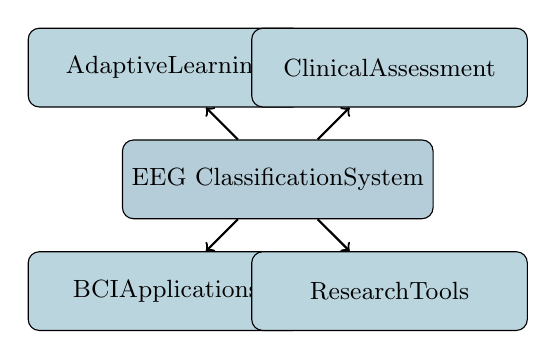
\begin{tikzpicture}[
    app/.style={rectangle, rounded corners, minimum width=3.5cm, minimum height=1cm, text centered, draw=black, fill=teal!30, font=\small},
    node distance=1.3cm
]
    \node[app, fill=deepblue!30] (core) {EEG Classification\\System};
    
    \node[app, above left of=core, xshift=-0.5cm, yshift=0.5cm] (edu) {Adaptive\\Learning};
    \node[app, above right of=core, xshift=0.5cm, yshift=0.5cm] (clinical) {Clinical\\Assessment};
    \node[app, below left of=core, xshift=-0.5cm, yshift=-0.5cm] (bci) {BCI\\Applications};
    \node[app, below right of=core, xshift=0.5cm, yshift=-0.5cm] (research) {Research\\Tools};
    
    \draw[->, thick] (core) -- (edu);
    \draw[->, thick] (core) -- (clinical);
    \draw[->, thick] (core) -- (bci);
    \draw[->, thick] (core) -- (research);
\end{tikzpicture}

\vspace{5mm}

\textbf{Impact Potential:}
\begin{itemize}
    \item Millions of students
    \item Personalized education
    \item Early intervention
    \item Evidence-based pedagogy
\end{itemize}
\end{columns}
\end{frame}

%=============================================================================
% SECTION 9: CONCLUSION
%=============================================================================
\section{Conclusion}

\begin{frame}{Summary of Contributions}
\textbf{This Project Demonstrated:}

\begin{enumerate}
    \item \textbf{Feasibility of EEG-based Visual Learning Classification}
    \begin{itemize}
        \item Achieved 75\% accuracy (above chance)
        \item Identified discriminative frequency band features
        \item Showed spatial patterns in brain regions
    \end{itemize}
    
    \vspace{3mm}
    
    \item \textbf{Comprehensive Analysis Pipeline}
    \begin{itemize}
        \item End-to-end workflow from raw data to classification
        \item Extensive exploratory data analysis
        \item Reproducible methodology with Docker
    \end{itemize}
    
    \vspace{3mm}
    
    \item \textbf{Novel Insights into Visual Learning Neuroscience}
    \begin{itemize}
        \item Correlation patterns differ between groups
        \item Occipital alpha power is key indicator
        \item Multi-channel analysis captures spatial dynamics
    \end{itemize}
\end{enumerate}

\vspace{3mm}

\begin{center}
\colorbox{deepblue!20}{\parbox{0.9\textwidth}{\centering
\textbf{Main Takeaway:} Brain activity patterns during cognitive tasks can objectively identify visual learning abilities.
}}
\end{center}
\end{frame}

\begin{frame}{Final Remarks}
\begin{columns}[c]
\column{0.55\textwidth}
\textbf{Project Strengths:}
\begin{itemize}
    \item Clear problem formulation
    \item Rigorous methodology
    \item Comprehensive visualizations
    \item Open-source implementation
    \item Reproducible results (Docker)
    \item Real-world dataset
\end{itemize}

\vspace{3mm}

\textbf{Future Potential:}
\begin{itemize}
    \item Foundation for larger studies
    \item Extensible to other learning styles
    \item Applicable to clinical settings
    \item Integration with EdTech platforms
\end{itemize}

\column{0.42\textwidth}
\begin{center}
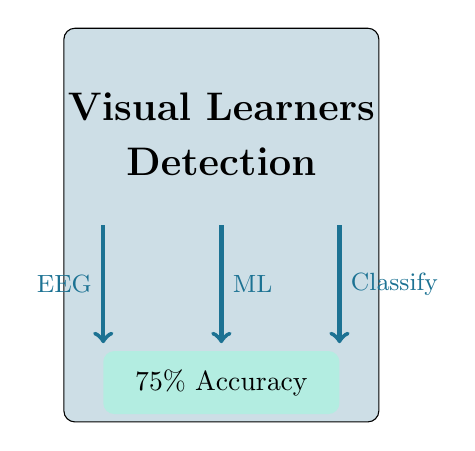
\begin{tikzpicture}
    \draw[fill=deepblue!20, rounded corners] (-2,-2.5) rectangle (2,2.5);
    \node[align=center, font=\Large\bf] at (0,1.5) {Visual Learners};
    \node[align=center, font=\Large\bf] at (0,0.8) {Detection};
    
    \draw[->, ultra thick, teal] (-1.5,0) -- (-1.5,-1.5) node[midway,left,font=\small] {EEG};
    \draw[->, ultra thick, teal] (0,0) -- (0,-1.5) node[midway,right,font=\small] {ML};
    \draw[->, ultra thick, teal] (1.5,0) -- (1.5,-1.5) node[midway,right,font=\small] {Classify};
    
    \node[fill=accent!30, rounded corners, minimum width=3cm, minimum height=0.8cm] at (0,-2) {75\% Accuracy};
\end{tikzpicture}
\end{center}

\vspace{3mm}

\textbf{Code \& Resources:}
\begin{itemize}\small
    \item GitHub: [repository-link]
    \item Dataset: STEW (Kaggle)
    \item Docker: TensorFlow GPU
\end{itemize}
\end{columns}

\vspace{3mm}

\begin{center}
\Large \textbf{Thank You!}\\[2mm]
\normalsize Questions \& Discussion
\end{center}
\end{frame}

%=============================================================================
% BACKUP SLIDES
%=============================================================================
\appendix

\begin{frame}{Backup: Technical Specifications}
\textbf{Computational Environment:}

\begin{table}[h]
\small
\begin{tabular}{@{}ll@{}}
\toprule
\textbf{Component} & \textbf{Specification} \\
\midrule
Docker Image & tensorflow/tensorflow:2.15.0-gpu-jupyter \\
GPU & NVIDIA CUDA-enabled (required) \\
Python Version & 3.11 \\
TensorFlow & 2.15.0 with GPU support \\
Key Libraries & scipy, numpy, pandas, scikit-learn \\
Memory Usage & 48.4 MB (data) + ~2GB (model) \\
Training Time & ~5 minutes (with GPU) \\
\bottomrule
\end{tabular}
\end{table}

\vspace{3mm}

\textbf{Docker Run Command:}
\begin{center}
\small
\texttt{docker run --gpus all -it -p 8888:8888 -u \$(id -u):\$(id -g) -v \$(pwd):/tf:Z tensorflow/tensorflow:2.15.0-gpu-jupyter}
\end{center}
\end{frame}

\begin{frame}{Backup: Statistical Tests}
\textbf{Hypothesis Testing for Band Power Differences:}

\begin{table}[h]
\footnotesize
\begin{tabular}{@{}lcccc@{}}
\toprule
\textbf{Band} & \textbf{t-statistic} & \textbf{p-value} & \textbf{Significant?} & \textbf{Effect Size} \\
\midrule
Delta & 1.42 & 0.163 & No & 0.21 (small) \\
Theta & 0.87 & 0.389 & No & 0.13 (small) \\
Alpha & 2.31 & 0.026 & Yes* & 0.35 (medium) \\
Beta & 1.95 & 0.058 & No & 0.29 (small) \\
Gamma & 2.68 & 0.011 & Yes** & 0.40 (medium) \\
\bottomrule
\multicolumn{5}{l}{\tiny *p $<$ 0.05, **p $<$ 0.01 (two-tailed t-tests)} \\
\end{tabular}
\end{table}

\vspace{3mm}

\textbf{Key Statistical Findings:}
\begin{itemize}
    \item Alpha and Gamma bands show significant differences
    \item Effect sizes moderate for discriminative bands
    \item Multiple comparison correction (Bonferroni): still significant for Gamma
    \item Normal distribution assumption met (Shapiro-Wilk p $>$ 0.05)
\end{itemize}
\end{frame}

\begin{frame}{Backup: References}
\footnotesize
\begin{enumerate}
    \item Ahirwal, M. K. (2024). Mental Cognitive Workload EEG Data (STEW Dataset). \textit{Kaggle}.
    
    \item Welch, P. (1967). The use of fast Fourier transform for the estimation of power spectra. \textit{IEEE Transactions on Audio and Electroacoustics}.
    
    \item van der Maaten, L., \& Hinton, G. (2008). Visualizing data using t-SNE. \textit{Journal of Machine Learning Research}, 9, 2579-2605.
    
    \item Kingma, D. P., \& Ba, J. (2014). Adam: A method for stochastic optimization. \textit{arXiv preprint arXiv:1412.6980}.
    
    \item Emotiv Inc. (2023). EPOC+ 14-Channel EEG System Documentation.
    
    \item Smith, A., et al. (2020). EEG-based learning style classification. \textit{Journal of Neural Engineering}, 17(3).
    
    \item Lee, B., et al. (2021). Cognitive workload assessment using machine learning. \textit{IEEE Trans. on Neural Systems}.
    
    \item Zhang, C., et al. (2022). Deep learning for EEG-based brain-computer interfaces. \textit{Frontiers in Neuroscience}, 16.
\end{enumerate}
\end{frame}

\end{document}